\chapter{Inflation}

The theory of cosmological inflation predicts that during very early times ($t\sim 10^{-36}$ s) the universe went through a phase of {\it exponential} expansion. The goal of this lecture is to describe the basic aspects of this theory, and to see how this conceptually simple idea provides a solution to some important problems in cosmology.

\section{The problems of the Standard Cosmological Model}

In the first ten lectures of this course we have outlined what is known as the {\it Standard Cosmological Model}, also known as the $\Lambda$CDM model. This model assumes an expanding universe described by general relativity with a FRW metric, which contains, in addition to normal matter (baryonic matter and radiation), contributions to the energy density in the forms of cold dark matter (CDM) and dark energy given by a cosmological constant ($\Lambda$). The $\Lambda$CDM model can explain all cosmological observations with high accuracy, including the abundances of hydrogen, helium, and other elements (as predicted by nucleosynthesis), the existence of the CMB (as predicted by recombination) and its anisotropies, the large-scale structure of the universe, and the late-time cosmic acceleration. Despite its enormous success, however, this model is unable to explain a number of important problems in cosmology. These problems (which are described in more detail below) are the following:
\begin{itemize}
\item {\bf The cosmological constant problem:} Why is the observed value of the cosmological constant so small?
\item {\bf The flatness problem:} Why is the universe flat (or very nearly so)?
\item {\bf The horizon problem:} Why is the universe so homogeneous and isotropic?
\item {\bf The monopole problem:} Why don't we observe magnetic monopoles?
\end{itemize}

\subsection{The cosmological constant problem}

This problem arises when we compare the observed value of the cosmological constant as inferred from the accelerated expansion of the universe, with the generic value predicted by quantum mechanics as we currently understand it. These two values turn out to be different by more than a hundred orders of magnitude!

The existence of a cosmological constant $\Lambda$ gives a contribution to the energy density of the universe that, as we have seen in past lectures, is constant in time (it is independent of the scale factor), and is given by
\begin{equation}
\rho_{\Lambda}=\frac{\Lambda c^2}{8\pi G}.
\end{equation}
Assuming that the late-time cosmic acceleration is indeed due to a cosmological constant (which is the most widely accepted explanation), then we can directly measure the value of $\rho_{\Lambda}$ from observations of type Ia supernovae (see lecture 10). We have seen that the present value of the dark energy density parameter is
\begin{equation}
\Omega_{\Lambda}(t_0)\equiv \frac{\rho_{\Lambda}}{\rho_c(t_0)}\simeq 0.7.
\end{equation}
For a present value of the critical density given by $\rho_c(t_0)\simeq 5.2\times10^{9}~\mathrm{eV~m^{-3}}$, this yields
\begin{equation}
\rho_{\Lambda}\simeq 4\times10^{9}~\mathrm{eV~m^{-3}}.
\end{equation}
In quantum mechanics, on the other hand, a cosmological constant gives an energy density that can be interpreted as the energy of the vacuum.\footnote{If you have studied the basics of quantum mechanics, you may know that stable systems possess a state of minimum energy, known as the {\it ground state}. The term ``vacuum'' is really just a fancy word for ground state that is used in the context of quantum field theory.} This vacuum energy can be calculated in the context of the Standard Model, with the result
\begin{equation} \label{eq:rho_vac}
\rho_{\mathrm{vac}}\sim 10^{133}~\mathrm{eV~m^{-3}}.
\end{equation}
We see that there is a difference of 124 orders of magnitude between $\rho_{\Lambda}$ and $\rho_{\mathrm{vac}}$! This problem is often referred to as the biggest disagreement between theory and experiment in the history of physics. We should emphazise, however, that the above value of $\rho_{\mathrm{vac}}$ is not a precise result, but rather a generic order-of-magnitude estimate. The precise value cannot be calculated exactly with our current knowledge of particle physics, and in principle it could be that $\rho_{\mathrm{vac}}$ turns out to be as small as what cosmological observations suggest. However, for that to be the case, there must be some extremely precise cancelations between the different contributions to $\rho_{\mathrm{vac}}$. We currently do not know of any physical mechanism that could explain why these cancelations happen, which means that the cosmological constant problem is a {\it naturalness problem}: although there is no physical law that prevents $\rho_{\mathrm{vac}}$ from being very small, having such a small value would be extremely unnatural.

The best ``solution'' to the cosmological constant problem is known as the {\it anthropic principle}: the cosmological constant $\Lambda$ must be extremely small because otherwise we (human beings) would not be here to formulate the problem in the first place. Indeed, if the dark energy density $\rho_{\Lambda}$ were as large as the generic quantum-mechanical prediction, eq.\ (\ref{eq:rho_vac}), then the dark energy would have become dominant at much earlier times, with the result that galaxies (and stars, planets, people, etc.) could not have formed. The problem with the anthropic principle is that it is not really a physical explanation (it is not based on a physical law or mechanism), which is why many physicists are not convinced, and the search for a physical solution to the cosmological constant problem remains one of the most active fields of research today.

\subsection{The flatness problem}

The flatness problem refers to the question of why is the universe almost perfectly flat. We will see in the following that, in the context of the $\Lambda$CDM model, we would generically expect the universe to be highly curved at the present time. We begin with the Friedmann equation,
\begin{equation} \label{eq:flatness_prob1}
\left(\frac{\dot{a}}{a}\right)^2=\frac{8\pi G}{3c^2}\rho(t)-\frac{kc^2}{R^2a^2},
\end{equation}
where $a(t)$ is the scale factor, $\rho(t)$ is the total energy density, $R$ is the radius of curvature of the universe, and $k$ is a constant equal to $0$, $+1$, or $-1$, depending on whether the universe is flat, positively curved, or negatively curved, respectively. Dividing eq.\ (\ref{eq:flatness_prob1}) by the Hubble parameter $H(t)=\dot{a}(t)/a(t)$, we obtain
\begin{equation} \label{eq:flatness_prob2}
1=\frac{\rho(t)}{\rho_c(t)}-\frac{kc^2}{R^2H^2a^2},
\end{equation}
where the critical density is defined as
\begin{equation}
\rho_c(t)=\frac{3c^2H(t)^2}{8\pi G}.
\end{equation}
Using the definition of the density parameter $\Omega(t)=\rho(t)/\rho_c(t)$ we can rewrite eq.\ (\ref{eq:flatness_prob2}) as
\begin{equation} \label{eq:flatness_prob3}
1-\Omega(t)=-\frac{kc^2}{R^2H(t)^2a(t)^2}.
\end{equation}
Next we evaluate this last equation at the present time, $t=t_0$, using that $H(t_0)\equiv H_0$ and $a(t_0)\equiv1$:
\begin{equation} \label{eq:flatness_prob4}
1-\Omega(t_0)=-\frac{kc^2}{R^2H_0^2}.
\end{equation}
Combining eqs.\ (\ref{eq:flatness_prob3}) and (\ref{eq:flatness_prob4}) we obtain
\begin{equation} \label{eq:flatness_prob7}
1-\Omega(t)=\big(1-\Omega(t_0)\big)\frac{H_0^2}{H(t)^2a(t)^2}.
\end{equation}
Let us focus on the early times, during the radiation-dominated era, for which the Friedmann equation approximately reads
\begin{equation} \label{eq:flatness_prob5}
H(t)^2=\frac{8\pi G}{3c^2}\rho_r(t),
\end{equation}
where $\rho_r(t)$ is the radiation energy density.

\par\vspace{\baselineskip}

{\bf Exercise.} Using eq.\ (\ref{eq:flatness_prob5}) and the fact that
\begin{equation}
\rho_r(t)=\frac{\rho_r(t_0)}{a(t)^4},
\end{equation}
show the following result:
\begin{equation} \label{eq:flatness_prob6}
\frac{H(t)^2}{H_0^2}=\frac{\Omega_r(t_0)}{a(t)^4},
\end{equation}
where $\Omega_r(t_0)$ is the radiation density parameter evaluated at the present time.

\par\vspace{\baselineskip}

Finally, using eq.\ (\ref{eq:flatness_prob6}) in eq.\ (\ref{eq:flatness_prob7}) we obtain
\begin{equation} \label{eq:flatness_prob8}
1-\Omega(t)=\big(1-\Omega(t_0)\big)\frac{a(t)^2}{\Omega_r(t_0)},
\end{equation}
a result that is valid during the radiation-dominated era. Recall from eq.\ (\ref{eq:flatness_prob3}) that the difference $\big(1-\Omega(t)\big)$ is inversely related to the radius of curvature $R$; the larger $R$ (that is, the flatter the universe), the closer is $\Omega(t)$ to unity. What eq.\ (\ref{eq:flatness_prob8}) then tells us is that the departure from perfect flatness decreases as we go back in time, since $a(t)$ (the only time-dependent quantity on the right-hand side of eq.\ (\ref{eq:flatness_prob8})) becomes smaller at earlier times. Experimentally, we have that\footnote{Here we are being conservative with the experimental errors; more recent data gives a smaller bound on $|1-\Omega(t_0)|$. However, this only makes the flatness problem worse.}
\begin{equation}
|1-\Omega(t_0)|<0.2,
\end{equation}
and that $\Omega_r(t_0)\simeq8\times10^{-5}$. We are now ready to evaluate eq.\ (\ref{eq:flatness_prob8}) during the radiation-dominated era. For instance, we may evaluate at the time of nucleosynthesis, $t=t_{\mathrm{nuc}}$, with a corresponding scale factor of $a(t_{\mathrm{nuc}})\simeq 4\times10^{-8}$, which implies that
\begin{equation} \label{eq:flatness_nucleosynthesis}
|1-\Omega(t_{\mathrm{nuc}})|=|1-\Omega(t_0)|\frac{a(t_{\mathrm{nuc}})^2}{\Omega_r(t_0)}<3\times10^{-14}.
\end{equation}
This result tells us that the universe was extremely flat at the time of recombination. Assuming that the universe was dominated by radiation all the way back to the Big Bang, then the earliest time at which we can evaluate eq.\ (\ref{eq:flatness_prob8}) corresponds to the {\it Planck time}: $t_P\simeq5\times10^{-44}$ s. This is the time at which general relativity starts to be applicable; before this time the energy density in the universe is so high that quantum effects become dominant, so that general relativity (which is a classical theory that neglects these quantum effects) breaks down and can no longer be trusted. Since the Friedmann equation follows from the Einstein equations, eq.\ (\ref{eq:flatness_prob8}) can be applied at the Planck time, but not at earlier times. Evaluating at $t=t_P$ we obtain the bound
\begin{equation} \label{eq:flatness_plancktime}
|1-\Omega(t_P)|<1\times10^{-60}.
\end{equation}
This means that, assuming the universe was radiation-dominated at the Planck time, $\Omega(t_P)$ must be equal to unity with an accuracy of one part in $10^{60}$. The reason why this is a problem is that the value of $\Omega(t_P)$ must be determined by what happens before the Planck time, and therefore it must presumably depend on {\it random} quantum effects. The fact that a random number turns out to be equal to unity with such a high accuracy is of course a huge, unnatural coincidence. This is the flatness problem, and we will see below that the problem arises from the incorrect assumption that the universe was radiation-dominated all the way back to the Planck time.

\subsection{The horizon problem}

Consider an observer at the present time, $t=t_0$. The most distant object she can in principle observe is one for which the light it emitted at $t=0$ (immediately after the Big Bang) is just reaching her at $t=t_0$. The distance to such an object is called the {\it horizon distance}, denoted by $d_h(t_0)$. We can think of $d_h(t_0)$ as the radius of a sphere that corresponds to the observable universe centered on the observer (fig.\ \ref{fig:lec12_2}); indeed, any signal from objects outside this sphere has not had enough time to reach the observer, simply because the universe has a finite age and because signals cannot travel faster than light. We can similarly define the horizon distance at any time, $d_h(t)$, by considering the size of the observable universe centered on an observer at a time $t$ after the Big Bang.
\begin{figure}[ht]
\begin{center}
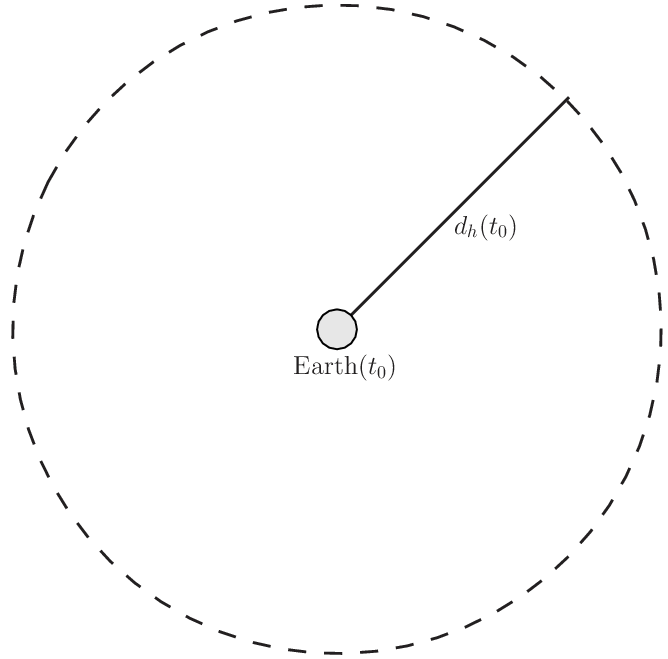
\includegraphics[scale=0.4]{Draw/lec12_2.png}
\end{center}
\caption{Horizon distance}
\label{fig:lec12_2}
\end{figure}

The precise relation between $d_h(t)$ and the time $t$ depends, of course, on how the universe has evolved during all times before $t$. If one assumes that the universe was radiation-dominated during the early times, and then became matter-dominated (recall that this is the picture in the $\Lambda$CDM model), then the following approximate relation holds during the matter-dominated epoch:
\begin{equation} \label{eq:horizon_dist_matter}
d_h(t)\simeq 3ct.
\end{equation}
With this result we can now evaluate $d_h(t)$ at different times. For instance, the present value of the horizon distance can be shown to be $d_h(t_0)\approx 1.4\times10^{10}\,{\mathrm{pc}}\approx14\,{\mathrm{Gpc}}$. Compare this with the horizon distance at the time of recombination, $t=t_{\mathrm{rec}}$, given by\footnote{Recall that recombination occurs during the matter-dominated era.}
\begin{equation}
d_h(t_{\mathrm{rec}})\simeq 0.4\,{\mathrm{Mpc}}.
\end{equation}

One more concept that we need to introduce is the {\it angular-diameter distance}. If an object of length $\Delta l$ subtends an angle $\theta$ to an observer (see fig.\ \ref{fig:lec12_3}), then the angular-diameter distance between the object and the observer is defined as
\begin{equation} \label{eq:ang_diam_dist}
d_A=\frac{\Delta l}{\theta}.
\end{equation}
You may argue that eq.\ (\ref{eq:ang_diam_dist}) is just the definition of the radian measure of the angle $\theta$. That would indeed be true in Euclidean space; however, in an expanding universe one has to be careful when measuring distances, and it is important to give a precise definition of what we mean when we speak of the distance between two objects.
\begin{figure}[ht]
\begin{center}
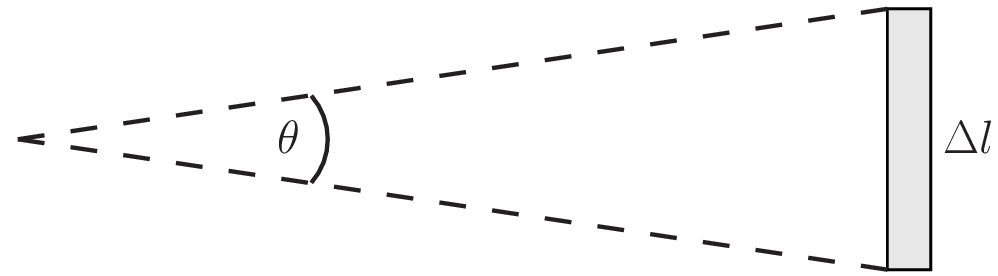
\includegraphics[scale=0.3]{Draw/lec12_3.png}
\end{center}
\caption{Angular-diameter distance}
\label{fig:lec12_3}
\end{figure}

We will denote by $d_A(t_{\mathrm{rec}})$ the angular-diameter distance from the Earth to the {\it surface of last scattering}, that is, the surface where the CMB photons come from. One can show that it has the value
\begin{equation}
d_A(t_{\mathrm{rec}})\simeq 13\,{\mathrm{Mpc}}.
\end{equation}

Consider two points separated by a horizon distance at the time of recombination, $t=t_{\mathrm{rec}}$. The angular separation $\theta_h$ between them, as seen on the CMB, can be found from eq.\ (\ref{eq:ang_diam_dist}):
\begin{equation} \label{eq:horizon_prob1}
\begin{split}
\theta_h&=\frac{d_h(t_{\mathrm{rec}})}{d_A(t_{\mathrm{rec}})}\\
&\simeq \frac{0.4\,{\mathrm{Mpc}}}{13\,{\mathrm{Mpc}}}\simeq 0.03\,{\mathrm{rad}}\simeq 2^{\circ}.
\end{split}
\end{equation}
This result tells us that two points on the CMB separated by more than about $2^{\circ}$ have a physical separation that is larger than a horizon distance. These two points are said to be {\it causally disconnected}, a concept that is illustrated in fig.\ \ref{fig:lec12_4}. We consider two CMB photons that were created, respectively, at the events $A$ and $B$ during recombination. In the graph of fig.\ \ref{fig:lec12_4} photons move along lines with slopes of $45^{\circ}$; since nothing can travel faster than light, this means that any information signal in this graph must correspond to a line that has a slope equal or larger than $45^{\circ}$. We have drawn two cones that extend from events $A$ and $B$ to the past, ending at $t=0$ (the Big Bang). These two cones represent the sets of events that could in principle have affected events $A$ and $B$. For example, event $C$ is inside the past cone of event $A$, meaning that it could have affected event $A$ but not event $B$; this is because any signal of information between $C$ and $B$ would have to travel faster than light, which is not possible. As another example, event $D$ does not belong to either past cone, so it cannot have affected either event $A$ or $B$. Since the past cones of events $A$ and $B$ do not overlap at all, no event before $t=t_{\mathrm{rec}}$ could have affected both $A$ and $B$, and the two events are said to be causally disconnected.
\begin{figure}[ht]
\begin{center}
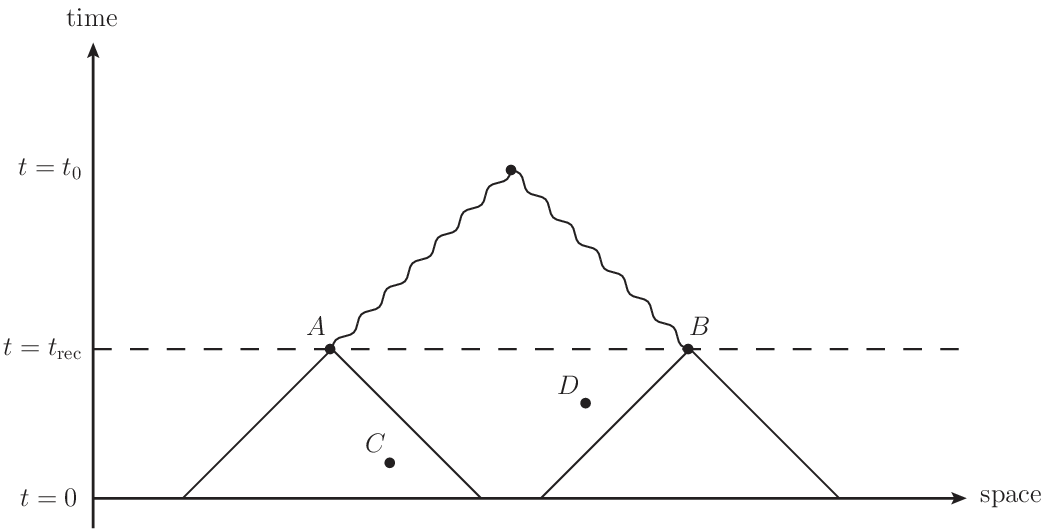
\includegraphics[scale=0.5]{Draw/lec12_4.png}
\end{center}
\caption{Causally disconnected regions}
\label{fig:lec12_4}
\end{figure}

Going back to eq.\ (\ref{eq:horizon_prob1}), we can divide the CMB into some $20,000$ patches of $2^{\circ}\times2^{\circ}$ that are all causally disconnected. Yet, all these $20,000$ patches have the same temperature with an accuracy of 1 part in $10^5$! Whatever are the processes that determined the temperature of one of these patches, they could not possibly have determined the temperature of any of the other patches, so how can it be that they all have roughly the same temperature? This is the horizon problem, which similarly to what happens in the flatness problem, arises from the incorrect assumption that the universe was radiation-dominated during the early times all the way back to the Big Bang.

\subsection{The monopole problem}

In nature we observe positive and negative electric charges, but not positive or negative magnetic charges, also known as {\it magnetic monopoles}. It is true that a magnet has a positive (``north'') and negative (``south'') magnetic poles; however, if you break the magnet in two you do not get isolated positive and negative poles, but instead you end up with two complete magnets, each one having a positive and a negative pole. The fact that magnetic monopoles are not found in nature has puzzled physicists since the time of Maxwell, who discovered that electric and magnetic fields are described by the same set of equations. In this sense, it seems odd that nature has provided us with elementary sources of electric fields (i.e.\ electric charges), but not of magnetic fields. One could argue that this is just a philosophical problem; unless there is a concrete physical reason to believe that magnetic monopoles should exist, there is no need to worry about the fact that they have not been observed. However, in the 1970's a strong physical reason arised from the studies of {\it Grand Unified Theories} (GUT).\footnote{We speak of Grand Unified Theories in plural because there exist a number of different candidate theories, none of which has been experimentally verified or falsified. However, these theories share several common properties and predictions which allows us to study them as a single class of theories in the context of cosmology.} These are theories that attempt to unify the three interactions of the Standard Model: the strong, the weak, and the electromagnetic interactions. One crucial and generic prediction of GUT theories is the existence of magnetic monopoles, which in theory should have been produced during the very early universe. We will see below that, according to the $\Lambda$CDM model, the abundance of magnetic monopoles should be extremely large, in obvious contradiction with observations. This is known as the monopole problem in cosmology.

First we would like to explain, very qualitatively, what is the nature of these magnetic monopoles, and why should we expect them to exist if some GUT theory is indeed realized in nature. In fig.\ \ref{fig:lec12_5} the four interactions of nature are shown how they become unified as the energy increases. We also show the temperature and time after the Big Bang at which the different unifications happen in the history of the universe. Going back in time, we first observe that the weak and electromagnetic interactions become unified at a temperature of $T\sim 10^{16}\,{\mathrm{K}}$; above this temperature, these two interactions manifest themselves as a single force known as the {\it electroweak} interaction. As we continue going back in time to higher temperatures, the strong and the electroweak forces become unified as well (in theory, since we cannot reach such high energies in particle accelerators), forming the so-called GUT interaction; theoretical calculations show that this unification occurs at a 
temperature of $T_{\mathrm{GUT}}\sim 10^{28}\,\mathrm{K}$, roughly $10^{-36}\,\mathrm{s}$ after the Big Bang. Many physicists believe that, if we continue to even higher temperatures, the force of gravity also becomes unified with the Standard Model forces, in what is known as the {\it theory of everything} (TOE); we will not be concerned with TOE here, since the details of how this unification happens are not well understood, and very few consistent candidate theories (string theory being perhaps the best one) have been proposed.
\begin{figure}[ht]
\begin{center}
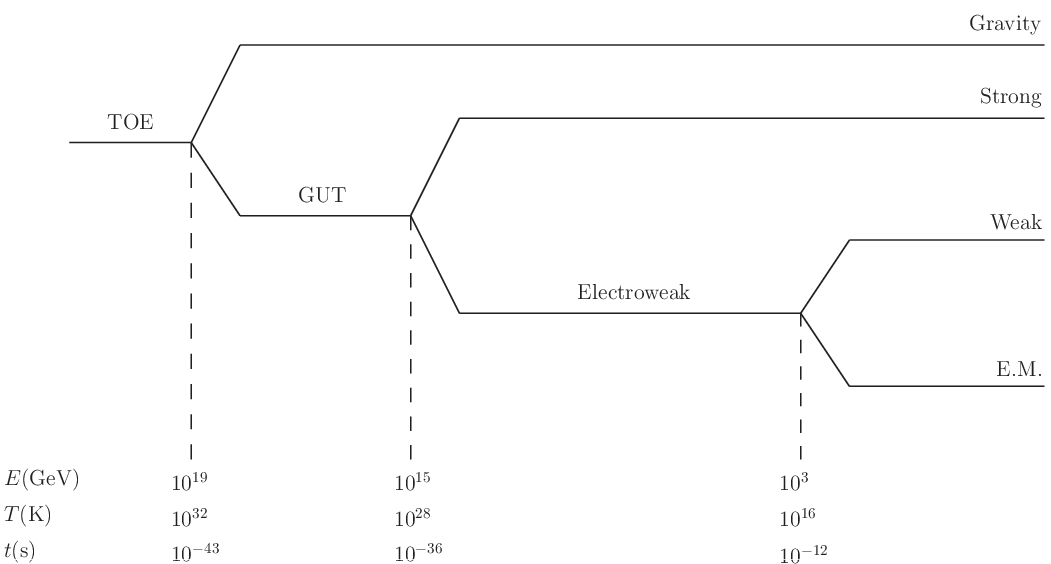
\includegraphics[scale=0.55]{Draw/lec12_5.png}
\end{center}
\caption{The four interactions of nature and their unification.}
\label{fig:lec12_5}
\end{figure}

We can think of $T_{\mathrm{GUT}}$ as the critical temperature of a phase transition. In general, a phase transition is a process in which a system changes discontinuously from one phase to another, each phase having its own characteristic properties. As an example, a magnet is characterized by a critical temperature $T_c$, below which the magnetic moments of the atoms in the magnet are all aligned in the same direction, giving the magnet a net magnetization. When the temperature $T$ of the magnet is increased from $T<T_c$ to $T>T_c$, the atoms' magnetic moments cease to be perfectly aligned and become randomly oriented, and as a result, the magnet loses its magnetization (see fig.\ \ref{fig:lec12_6}). One general property of phase transitions is that the high-temperature phase ($T>T_c$) is more {\it symmetric} than the low-temperature phase ($T<T_c$). In the example of the magnet, in the high-temperature phase the atoms' magnetic moments are randomly oriented with no preferred orientation, while in the low-temperature phase that symmetry is lost because the alignment of the atoms defines a preferred direction in the system. Something completely analogous happens at the GUT temperature: above $T_{\mathrm{GUT}}$ we have symmetric phase consisting of a single interaction, while below $T_{\mathrm{GUT}}$ the strong and electroweak forces are inequivalent and the symmetry is lost.
\begin{figure}[ht]
\begin{center}
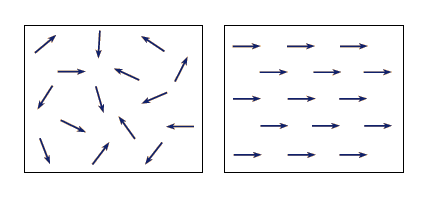
\includegraphics[scale=0.7]{Draw/lec12_6.png}
\end{center}
\caption{Phase transition in a magnet}
\label{fig:lec12_6}
\end{figure}

To describe the degree of symmetry of a system more quantitatively, we define a function called the {\it order parameter}, denoted by $\phi$. The order parameter is defined such that
\begin{itemize}
\item [] $\phi=0$ in the symmetric phase ($T>T_c$), and
\item [] $\phi=\pm \phi_0$ in the asymmetric phase ($T<T_c$),
\end{itemize}
where $\phi_0$ is some positive constant. As an example, consider a magnet that can be magnetized only along the vertical direction, either up or down. The order parameter in this case would correspond precisely to the value of the magnetization; in the high-temperature phase we have $\phi=0$, that is no net magnetization, while in the low-temperature phase the magnetization can take either of two values depending on whether it points up or down.

Suppose we start with a system initially at $T>T_c$, so that $\phi=0$ everywhere on the system. If we then lower the temperature down to $T_c$, we know that the system will undergo a phase transition and the order parameter will acquire either of the values $\pm\phi_0$. The question is, which one? The answer is that either $+\phi_0$ or $-\phi_0$ will occur with equal probabilities. However, it is not necessary that all points in the system acquire a single value of $\phi$; it is perfectly possible that some regions of the system have $+\phi_0$ while others have $-\phi_0$. And in fact, this will generally be the case whenever the system has more than one causally disconnected regions. Indeed, if two causally disconnected regions in a system undergo a phase transition, there is no reason why in the two of them $\phi$ should acquire the same value.
\begin{figure}[ht]
\begin{center}
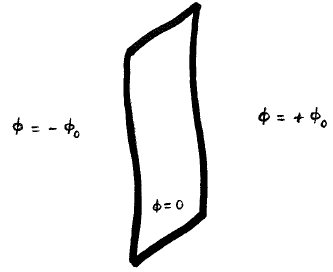
\includegraphics[scale=0.6]{Draw/lec12_7.png}
\end{center}
\caption{Domain wall}
\label{fig:lec12_7}
\end{figure}

Consider then two regions in the system, one with $\phi=+\phi_0$ and the other with $\phi=-\phi_0$. What happens on the surface that separates these two regions? Because the order parameter is a continuous function, it must have the value $\phi=0$ on the surface, even though the system is below the critical temperature (fig.\ \ref{fig:lec12_7}). Such a surface is called a {\it domain wall}. Fig.\ \ref{fig:lec12_1} shows a picture of some domain walls in a magnetic material made of nickel.
\begin{figure}[ht]
\begin{center}
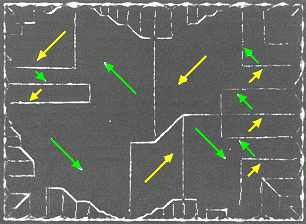
\includegraphics[scale=0.75]{Draw/lec12_1.png}
\end{center}
\caption{Domain walls (Image source: \url{http://www.tf.uni-kiel.de/matwis})}
\label{fig:lec12_1}
\end{figure}

Next we generalize the above to a system that has two order parameters $\phi_1$ and $\phi_2$. In this case the order parameters have the following properties:
\begin{itemize}
\item [] $\phi_1=\phi_2=0$ in the symmetric phase ($T>T_c$), and
\item [] $\phi_1^2+\phi_2^2=\phi_0^2$ in the asymmetric phase ($T<T_c$),
\end{itemize}
where $\phi_0$ is some positive constant. Thus, in this case there are infinite possibilities (all having equal probabilities) for the values of $\phi_1$ and $\phi_2$ in the asymmetric phase, defined by a circle of radius $\phi_0$ on the $\phi_1-\phi_2$ plane. We imagine again that a system of this type starts at $T>T_c$, and that we lower the temperature down to $T_c$. Again, if the system possess more than one causally disconnected regions, then some region will acquire a set of values $(\phi_1,\phi_2)$, while some other region will acquire a different set of values, although in every case we will have that $\phi_1^2+\phi_2^2=\phi_0^2$. However, an exception to this occurs when four regions with $(\phi_1>0,\phi_2>0)$, $(\phi_1<0,\phi_2>0)$, $(\phi_1>0,\phi_2<0)$, and $(\phi_1<0,\phi_2<0)$, intersect with each other along a curve where, by continuity, we must have $\phi_1=\phi_2=0$ (see fig.\ \ref{fig:lec12_8}). Such a curve is known as a {\it cosmic string}, and it is the one-dimensional analog of the 
domain wall for a system with two order parameters.
\begin{figure}[ht]
\begin{center}
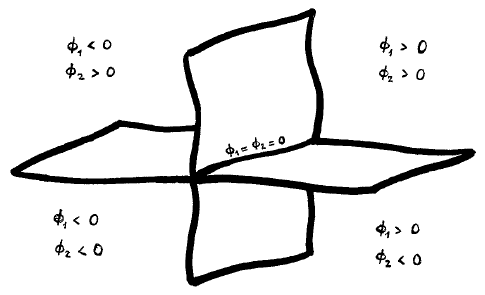
\includegraphics[scale=0.6]{Draw/lec12_8.png}
\end{center}
\caption{Cosmic string}
\label{fig:lec12_8}
\end{figure}

Finally, let us generalize the above to a system with three order parameters $\phi_1$, $\phi_2$, and $\phi_3$, with the properties that
\begin{itemize}
\item [] $\phi_1=\phi_2=\phi_3=0$ in the symmetric phase ($T>T_c$), and
\item [] $\phi_1^2+\phi_2^2+\phi_3^2=\phi_0^2$ in the asymmetric phase ($T<T_c$),
\end{itemize}
where $\phi_0$ is some positive constant. You can convince yourself, by going through the argument for the two-parameter case, that now there are eight possibilities for the signs of $(\phi_1,\phi_2,\phi_3)$. A system of this type with more than one causally disconnected regions may have all these eight regions intersecting at a single point, in which we must have that $\phi_1=\phi_2=\phi_3=0$ by continuity (see fig.\ \ref{fig:lec12_9}). Such a point is called a {\it monopole}, and corresponds to the zero-dimensional analog of the domain wall and the cosmic string. This is in fact the type of system described by GUT theories, and one can show that the monopole corresponding to the GUT phase transition generates a magnetic field very much like an electric charge generates an electric field, hence the name magnetic monopole. Domain walls, cosmic strings, and monopoles are examples of a class of objects known as {\it topological defects}.
\begin{figure}[ht]
\begin{center}
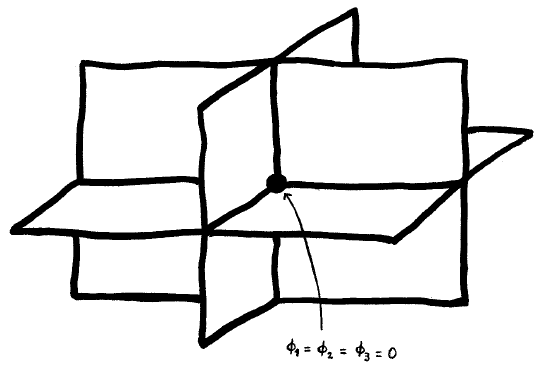
\includegraphics[scale=0.6]{Draw/lec12_9.png}
\end{center}
\caption{Monopole}
\label{fig:lec12_9}
\end{figure}

To summarize, we have shown qualitatively that whenever a phase transition occurs in a system with several causally disconnected regions, we expect in general that topological defects will be created. Let us apply this to the GUT phase transition that occured at $t=t_{\mathrm{GUT}}\sim 10^{-36}\,{\mathrm{s}}$ after the Big Bang. In this case the ``system'' is the universe itself, and we have seen that the corresponding topological defect is a magnetic monopole. The relevant question is, how many monopoles per unit volume should we expect to be created? We have seen that causally disconnected regions are separated by distances larger than $d_h(t)$, the horizon distance. This means that we should expect that roughly one magnetic monopole be created per horizon volume, which is of order $d_h(t)^3$. Then the number density of monopoles (number of monopoles per unit volume) created during the GUT phase transition is given by\footnote{Here and in the following the symbol ``$\sim$'' means that we are just making an 
order-of-magnitude estimate, and not a precise approximation.}
\begin{equation}
n_{\mathrm{mon}}(t_{\mathrm{GUT}})\sim \frac{(\mathrm{1\,monopole})}{(\mathrm{horizon~volume})}\sim \frac{1}{d_h(t_{\mathrm{GUT}})^3}.
\end{equation}
If we assume that the universe was dominated by radiation during the GUT phase transition, then one can show that
\begin{equation} \label{eq:horizon_dist_rad}
d_h(t_{\mathrm{GUT}})\simeq 2ct_{\mathrm{GUT}},
\end{equation}
which implies that
\begin{equation} \label{eq:monopole_prob1}
n_{\mathrm{mon}}(t_{\mathrm{GUT}})\sim 10^{82}\,\mathrm{m^{-3}}.
\end{equation}
The energy density of the magnetic monopoles can be estimated from their rest energy:\footnote{Although at $t=t_{\mathrm{GUT}}$ the monopoles have a sizeable kinetic energy that cannot be neglected, they soon become nonrelativistic, and the rest energy gives the correct order of magnitude of the total energy of a monopole.}
\begin{equation} \label{eq:monopole_prob2}
\rho_{\mathrm{mon}}(t_{\mathrm{GUT}})\sim (m_{\mathrm{mon}}c^2)n_{\mathrm{mon}}(t_{\mathrm{GUT}}),
\end{equation}
where $m_{\mathrm{mon}}$ is the mass of a magnetic monopole. One can show that the rest energy of a monopole is of the order of the energy at which GUT unification happens, that is $m_{\mathrm{mon}}c^2\sim E_{\mathrm{mon}}\sim10^{15}\,{\mathrm{GeV}}$. With this estimate one obtains from eqs.\ (\ref{eq:monopole_prob1}) and (\ref{eq:monopole_prob2}),
\begin{equation}
\rho_{\mathrm{mon}}(t_{\mathrm{GUT}})\sim 10^{97}\,\mathrm{GeV/m^3}.
\end{equation}
This energy density is several orders of magnitude smaller than the energy density of the radiation at that time, given by $\rho_r(t_{\mathrm{GUT}})\sim 10^{107}\,\mathrm{GeV/m^3}$, consistent with the assumption that the universe was dominated by radiation at the time of the GUT transition. The problem arises from the fact that the monopoles become nonrelativistic soon after this time, implying that their energy density decreases in time as
\begin{equation}
\rho_{\mathrm{mon}}(t)\propto \frac{1}{a(t)^3},
\end{equation}
for $t$ soon after $t_{\mathrm{GUT}}$. On the other hand, the energy density of the radiation always decreases as $\rho_r\propto 1/a^4$, meaning that at some point the energy density of the universe will become dominated by the magnetic monopoles. One can show that, under the above assumptions, this occurs at a time of roughly $10^{-16}\,\mathrm{s}$. This is much earlier than the time of nucleosynthesis ($t\sim 200\,\mathrm{s}$), which we know happened when the universe was radiation-dominated. Morover, according to this the universe should be dominated by monopoles today, which is obviously not the case. Similarly to what happens in the horizon problem, we will see that the monopole problem arises from assuming an incorrect expression for the horizon distance.

\section{The theory of inflation}

The theory of cosmological inflation was proposed in 1980 by Alan Guth as a possible solution to the flatness, horizon, and monopole problems. Although inflation has not been verified experimentally, there exists some compelling indirect evidence that supports it, which will likely be improved by experiments during the next few years. Inflation states that there was a period during the very early universe in which the rate of expansion was exponential:
\begin{equation} \label{eq:inflation_scalefactor}
a(t)=a(t_i)e^{H_I(t-t_i)}.
\end{equation}
Here $H_I$ is the Hubble parameter during inflation (which is assumed to be constant), and $t_i$ is the time at which inflation started. We expect that the mechanism responsible for inflation is somehow related to the physics of GUT. This is because inflation has to be driven by some new field or fields, and we know that whenever a phase transition takes place new fields become relevant at higher energies.\footnote{In the case of the electroweak unification, these new fields correspond to the $W$ and $Z$ bosons.} If this is the case, then we can make a rough estimate for $H_I$ and $t_i$ simply by dimensional analysis. The initial time $t_i$ must be related to the only characteristic timescale of GUT, namely $t_{\mathrm{GUT}}$, while the Hubble parameter must be related to $t_{\mathrm{GUT}}^{-1}$ since it has dimensions of inverse time:
\begin{equation}
\begin{split}
t_i&\sim t_{\mathrm{GUT}}\sim 10^{-36}\,{\mathrm{s}},\\
H_I&\sim t_{\mathrm{GUT}}^{-1}\sim 10^{36}\,{\mathrm{s^{-1}}}.
\end{split}
\end{equation}
Suppose that inflation ends at a time $t_f\sim 100t_i\sim 10^{-34}\,\mathrm{s}$, after which the universe becomes radiation-dominated and begins to evolve according to the standard $\Lambda$CDM model. From the time $t_i$ to $t_f$ the universe then expands by a factor of
\begin{equation}
\begin{split}
\frac{a(t_f)}{a(t_i)}&=e^{H_I(t_f-t_i)}\\
&\sim e^{100}\sim 10^{43}.
\end{split}
\end{equation}
The time $t_f$ is still much earlier than the time of quark confinement, neutrino decoupling, and all the other phases of the thermal history of the universe that are well understood,\footnote{The thermal history of the universe was studied in chapters 6 and 7.} so everything we have said in the past eleven lectures remains valid. We are now ready to see how inflation provides a simple solution to the flatness, horizon, and monopole problems.

\subsection{Solution to the flatness problem}

In the previous section we showed that the Friedmann equation implies that
\begin{equation}
1-\Omega(t)=-\frac{kc^2}{R^2H(t)^2a(t)^2}.
\end{equation}
Taking the absolute value of this equation gives\footnote{Here we are implicitly assuming that the $k\neq0$, so that the universe is assumed not to be perfectly flat (which would be unnatural from a physical point of view). However, the flat case can be formally obtained by taking the limit $R\to\infty$ in eq.\ (\ref{eq:sol_flatness_prob1}).}
\begin{equation} \label{eq:sol_flatness_prob1}
|1-\Omega(t)|=\frac{c^2}{R^2H(t)^2a(t)^2}.
\end{equation}
To apply this equation during inflation, we take $H(t)=H_I$ and $a(t)=a(t_i)e^{H_I(t-t_i)}$. Then, evaluating the quantity $|1-\Omega(t)|$ at the end and at the beginning of inflation, yields the ratio
\begin{equation}
\begin{split}
\frac{|1-\Omega(t_f)|}{|1-\Omega(t_i)|}&=\frac{a(t_i)^2}{a(t_f)^2}=e^{-2H_I(t_f-t_i)}\\
&\sim e^{-200}\sim 10^{-87}.
\end{split}
\end{equation}
Suppose the universe was highly curved before inflation, say $|1-\Omega(t_i)|\sim 1$, which is what we would expect if the initial value of $\Omega(t)$ was determined by random quantum effects. Then, at the end of inflation we will have
\begin{equation}
|1-\Omega(t_f)|\sim 10^{-87}.
\end{equation}
This is more than enough to explain why the universe is so flat at the present time; see eqs.\ (\ref{eq:flatness_nucleosynthesis}) and (\ref{eq:flatness_plancktime}). We see that the exponential expansion of inflation produces an extremely flat universe by reducing the effects of the curvature by many orders of magnitude.

\subsection{Solution to the horizon problem}

The solution to the horizon problem is very simple. We have seen in the previous section that, assuming that the universe was radiation-dominated in the early times all the way back to the Big Bang, then the horizon distance $d_h(t)$ would have grown proportional to $ct$ from the beginning; see eqs.\ (\ref{eq:horizon_dist_matter}) and (\ref{eq:horizon_dist_rad}). Inflation changes this picture completely, since the exponential expansion implies that the horizon distance grows exponentially, rather than linearly, in time:
\begin{equation}
d_h(t)\sim ct_i e^{H_I(t-t_i)},
\end{equation}
so that by the end of inflation the horizon distance is
\begin{equation}
d_h(t_f)\sim ct_i e^{100}\sim 10^{16}\,{\mathrm{m}}\sim 1\,{\mathrm{pc}}.
\end{equation}
With this result one can now compute the horizon distance at the time of recombination, with the result
\begin{equation}
d_h(t_{\mathrm{rec}})\sim 10^{43}\,{\mathrm{Mpc}}.
\end{equation}
Compare this to the value of $\sim 0.4\,\mathrm{Mpc}$ we would obtain in the absence of inflation. Thus, we see that the horizon problem arises from using an incorrect, much smaller value of the horizon distance at the time of recombination. The photons of the CMB do not really come from several thousand causally disconnected regions, but they actually come from a single one, and it is therefore not surprising that they all have approximately the same temperature.

\subsection{Solution to the monopole problem}

Intuitively, we expect inflation to dilute the magnetic monopoles created during the GUT phase transition, hopefully reducing their number density to a very low level, explaining why they have not been detected and why they seem to have not played any role in the thermal history of the universe. We will see next that this is precisely what happens.

Suppose that the GUT phase transition roughly coincides with the beginning of inflation, so that $t_i\sim t_{\mathrm{GUT}}$. This is consistent with the assumption that the mechanism of inflation is somehow related to the physics of GUT. Then from eq.\ (\ref{eq:monopole_prob1}) we have
\begin{equation}
n_{\mathrm{mon}}(t_i)\sim 10^{82}\,{\mathrm{m^{-3}}}
\end{equation}
for the number density of magnetic monopoles. We have argued that the monopoles become nonrelativistic soon after they are produced, so that we expect that $n_{\mathrm{mon}}\propto 1/a^3$ during inflation. Then, using eq.\ (\ref{eq:inflation_scalefactor}), we can compute the number density of monopoles at the end of inflation:
\begin{equation}
\begin{split}
n_{\mathrm{mon}}(t_f)&\sim \left(e^{H_I(t_f-t_i)}\right)^{-3}n_{\mathrm{mon}}(t_i)\\
&\sim e^{-300}\,10^{82}\,{\mathrm{m^{-3}}}\sim 5\times 10^{-49}\,{\mathrm{m^{-3}}}
\end{split}
\end{equation}
In order to compute the present abundance of magnetic monopoles we need to consider the additional (standard) expansion from $t=t_f$ (end of inflation) until $t=t_0$ (today). This gives
\begin{equation}
n_{\mathrm{mon}}(t_0)\sim 10^{-61}\,{\mathrm{m^{-3}}}.
\end{equation}
This is such a small number that the probability of finding even a single monopole in our galaxy is essentially zero. This is good news, because it solves the monopole problem, explaining why don't we observe magnetic monopoles in nature. But in another sense it is bad news, because this result tells us that, if they actually exist, we are not going to ever observe them. The only hope would be to produce them, or at least to infer their existence, from experiments in particle accelerators. However, if monopoles have the very large mass that GUT theories predict, then particle accelerators are not going to reach the required energies any time soon. In this sense, the best hope would be to find other, more indirect experimental signatures for GUT and its properties.

\subsection{Conclusions}

We have seen that inflation provides a simple solution to the flatness, horizon, and monopole problems of cosmology. However, there are many aspects of this theory that we have not mentioned. Indeed, inflation has been one of the most active fields of research for the past three decades, and describing it in detail would probably require an entire course. On the theoretical side, we have not explained what are the possible physical mechanisms that could produce an inflationary expansion, or how these mechanisms are related to GUT or perhaps other more exotic theories. On the experimental side, we have said little about the possible observational signatures of inflation, and how cosmologists hope to either verify or falsify this theory with the present and future generations of experiments.